% !TEX program = xelatex
\documentclass[11pt, a4paper]{article}
\usepackage{fontspec}
\usepackage{Alegreya}
\usepackage{AlegreyaSans}
\usepackage{polyglossia}
\setdefaultlanguage{french}
\usepackage[top=1.7cm, bottom=1.7cm, left=2cm, right=2cm]{geometry}
\usepackage{amsmath}
\usepackage{graphicx}
\usepackage{booktabs}
\usepackage{xcolor}
\definecolor{navy}{HTML}{00578A}
\definecolor{navymed}{HTML}{1D7AAE}
\definecolor{gray2}{HTML}{444444}
\definecolor{light}{HTML}{EAF3F8}
\definecolor{gold}{HTML}{6B5A2C}
\definecolor{vert}{HTML}{1E8449}
\definecolor{rouge}{HTML}{C0392B}
\usepackage{enumitem}
\setlist[itemize]{leftmargin=1.2em, itemsep=1.5pt, topsep=2pt, label=\textcolor{navymed}{\small\textbullet}}
\usepackage{hyperref}
\hypersetup{colorlinks=true, urlcolor=navy, linkcolor=navy}
\setlength{\parindent}{0pt}\setlength{\parskip}{4pt}
\pagestyle{plain}
\newcommand{\rub}[1]{\vspace{4pt}{\AlegreyaSansMedium\large\color{navy}\MakeUppercase{#1}}\par
  \vspace{1pt}{\color{navy}\rule{\linewidth}{1.4pt}}\par\vspace{3pt}}
\newcommand{\ssrub}[1]{\vspace{2pt}{\bfseries\color{navymed}#1}\par}

\begin{document}

\begin{center}
{\AlegreyaSansMedium\LARGE\color{navy} TerangaScore}\\[2pt]
{\large Documentation technique du prototype}\\[2pt]
{\small\color{gray2}Scoring de microcredit interpretable et analyse de survie, cooperatives financieres de l'UEMOA}\\[1pt]
{\small\color{gray2}Equipe TERANGALAB, Hackathon national CIF, projet DigiCoop-WA+}
\end{center}
{\color{navy}\rule{\linewidth}{2pt}}

\rub{1. Contexte et solution}
Dans les Systemes Financiers Decentralises (SFD) de l'UEMOA, l'octroi de microcredit repose souvent sur une analyse manuelle, subjective et longue. \textbf{TerangaScore} automatise et objective cette decision, avec deux moteurs complementaires et \textbf{interpretables} :
\begin{itemize}
  \item une \textbf{scorecard} (probabilite de defaut) qui repond a : \emph{ce client va-t-il faire defaut ?} ;
  \item une \textbf{analyse de survie} qui repond a : \emph{quand} le defaut risque-t-il de survenir ?
\end{itemize}
L'interpretabilite complete repond aux exigences prudentielles de la BCEAO (decision justifiable, opposable).

\rub{2. La base de donnees}
Base synthetique calibree sur la realite UEMOA : \textbf{5 000 clients}, \textbf{32 variables}. Elle couvre le socio-demographique (pays, zone, sexe, age, instruction), l'activite (secteur, revenu), la relation cooperative (anciennete, historique, epargne), le credit (montant, duree, taux, mensualite, taux d'effort), les \textbf{donnees alternatives} (mobile money), et les variables de survie.
\begin{itemize}
  \item Cible binaire : \texttt{defaut} (taux de defaut \textbf{11,8\%}).
  \item Variables de survie : \texttt{duree\_observation\_mois} (temps jusqu'au defaut ou censure) et \texttt{evenement\_defaut}.
\end{itemize}
Formats disponibles : \texttt{.csv}, \texttt{.dta} (Stata), \texttt{.rds} (R).

\rub{3. Methodologie de la scorecard}
\ssrub{WOE, Weight of Evidence}
Chaque classe $i$ d'une variable est transformee en force de preuve du defaut :
\[
\text{WOE}_i = \ln\!\left( \frac{\%\ \text{bons}_i}{\%\ \text{mauvais}_i} \right)
\]
\ssrub{IV, Information Value (pouvoir predictif)}
\[
\text{IV} = \sum_i \left( \%\ \text{bons}_i - \%\ \text{mauvais}_i \right)\times \text{WOE}_i
\]
\ssrub{Regression logistique et mise en points}
Une regression logistique est ajustee sur les variables en WOE, puis convertie en points :
\[
\text{Score} = \text{Offset} + \text{Factor}\times \ln(\text{odds}),\qquad
\text{Factor} = \frac{\text{PDO}}{\ln(2)}
\]
Chaque modalite rapporte des points : la decision est \textbf{explicable ligne par ligne}. Le binning et les WOE sont appris \textbf{sur l'echantillon d'apprentissage uniquement} (anti-fuite).

\rub{4. Resultats du scoring}
Performance sur l'echantillon de test (1 500 clients) :

\begin{center}
\begin{tabular}{lcc}
\toprule
\textbf{Indicateur} & \textbf{Valeur} & \textbf{Lecture} \\
\midrule
AUC  & \textbf{0,847} & bon ($>0{,}8$) \\
Gini & \textbf{0,694} & fort ($>0{,}4$) \\
KS   & \textbf{0,542} & fort ($>0{,}3$) \\
\bottomrule
\end{tabular}
\end{center}

\ssrub{Variables les plus predictives (IV)}
\begin{center}
\small
\begin{tabular}{lc l c}
\toprule
Variable & IV & Variable & IV \\
\midrule
Taux d'effort & 1,006 & Historique de remboursement & 0,297 \\
Ratio epargne/credit & 0,623 & Anciennete de membre & 0,220 \\
Duree du credit & 0,448 & Credits anterieurs & 0,177 \\
Mensualite & 0,352 & Revenu mensuel & 0,153 \\
Epargne moyenne & 0,345 & Secteur d'activite & 0,076 \\
\bottomrule
\end{tabular}
\end{center}

\ssrub{Exemple de scorecard (variable : taux d'effort)}
\begin{center}
\small
\begin{tabular}{lc}
\toprule
Classe de taux d'effort & Points \\
\midrule
$\le 0{,}26$ (faible) & \textbf{63,6} \\
$0{,}26$ a $0{,}38$ & 51,5 \\
$0{,}38$ a $0{,}52$ & 42,8 \\
$0{,}52$ a $0{,}78$ & 33,5 \\
$>0{,}78$ (eleve) & \textbf{12,2} \\
\bottomrule
\end{tabular}
\end{center}
Plus le taux d'effort est eleve, moins le client obtient de points : logique metier respectee.

\rub{5. Analyse de survie du risque}
Au-dela de la decision binaire, l'analyse de survie modelise le \textbf{temps} jusqu'au defaut, en gerant la \textbf{censure} (credits arrives a terme sans defaut).

\begin{center}
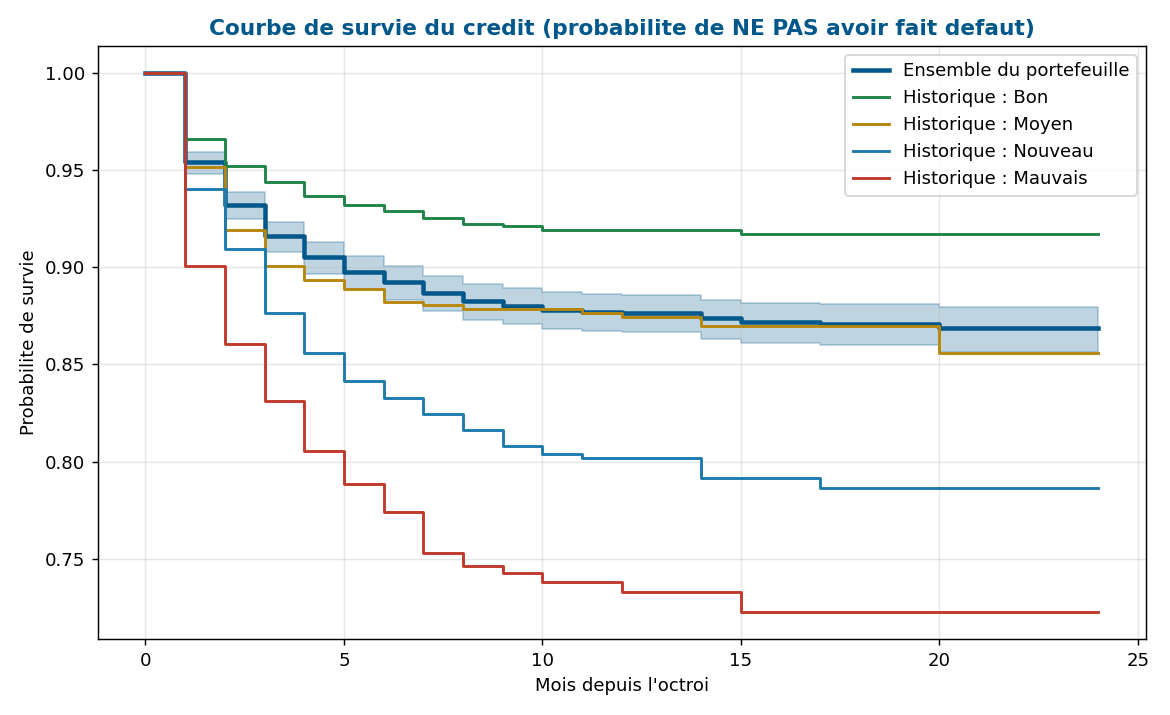
\includegraphics[width=0.88\linewidth]{courbe_survie.png}
\end{center}

\ssrub{Kaplan-Meier}
Survie du portefeuille : \textbf{91,6\%} a 3 mois, \textbf{89,2\%} a 6 mois, \textbf{87,6\%} a 12 mois. Le test du log-rank confirme des survies tres differentes selon l'historique ($p \approx 2\times 10^{-33}$) : les mauvais payeurs font defaut \textbf{plus tot et plus souvent}.

\ssrub{Modele de Cox (hazards proportionnels)}
Concordance (c-index) = \textbf{0,876} (analogue de l'AUC pour la survie). Hazard ratios (HR) :

\begin{center}
\small
\begin{tabular}{lc l c}
\toprule
Facteur de risque (\textcolor{rouge}{HR $>1$}) & HR & Facteur protecteur (\textcolor{vert}{HR $<1$}) & HR \\
\midrule
Historique Mauvais & 2,88 & Revenu mensuel & 0,81 \\
Taux d'effort & 2,20 & Epargne moyenne & 0,81 \\
Historique Nouveau & 1,56 & Anciennete de membre & 0,83 \\
Historique Moyen & 1,26 & Credits anterieurs & 0,85 \\
Secteur agricole & 1,25 & Credit solidaire & 0,88 \\
\bottomrule
\end{tabular}
\end{center}
Lecture : un historique \emph{Mauvais} multiplie par \textbf{2,9} le risque instantane de defaut ; l'\textbf{epargne} et l'\textbf{anciennete} le reduisent.

\rub{6. Interpretabilite et conformite BCEAO}
Les deux moteurs sont \textbf{transparents} : points par modalite pour la scorecard, hazard ratios pour la survie. Pour chaque decision, TerangaScore fournit la contribution de chaque variable, ce qui rend la decision \textbf{justifiable au membre et au superviseur}. C'est le pilier de conformite prudentielle.

\rub{7. Interoperabilite : API REST, securite et mode hors ligne}
Le moteur est expose via une \textbf{API REST} (FastAPI), pour que le systeme d'information d'une caisse (SFD) obtienne une decision par un simple appel HTTP/JSON, sans connaitre les details du modele. L'appli Streamlit et l'API partagent \textbf{le meme moteur} (aucune duplication de logique).

\ssrub{Points d'acces}
\begin{center}
\small
\begin{tabular}{l l l}
\toprule
Methode et route & Role & Acces \\
\midrule
\texttt{GET /health} & disponibilite du service & libre \\
\texttt{GET /modele/info} & qualite du modele (AUC, Gini, KS) & libre \\
\texttt{POST /score} & score, decision, explication & cle d'API \\
\texttt{POST /survie} & courbe de survie individuelle & cle d'API \\
\texttt{POST /evaluation} & score et survie en un appel & cle d'API \\
\texttt{GET /journal/statistiques} & suivi du portefeuille & cle d'API \\
\bottomrule
\end{tabular}
\end{center}
Une documentation interactive (Swagger) est generee automatiquement sur \texttt{/docs}.

\ssrub{Securite}
Les points d'acces de decision exigent une \textbf{cle d'API} (entete \texttt{X-API-Key}). Un appel sans cle ou avec une cle invalide est refuse (code \texttt{401}). Les entrees sont \textbf{validees} (age entre 18 et 100 ans, taux plafonne a 24\%, le taux d'usure BCEAO), ce qui protege le modele des donnees aberrantes.

\ssrub{Mode hors ligne et piste d'audit}
Chaque decision est \textbf{journalisee localement} dans une base SQLite, sans dependance reseau : une caisse sur un poste modeste et sans connexion permanente conserve une \textbf{piste d'audit} (tracabilite exigee par la BCEAO) et produit des statistiques de portefeuille (taux d'acceptation, montant total accorde, score moyen).

\rub{8. Architecture et maturite}
\begin{itemize}
  \item \textbf{Realise} : base UEMOA, scorecard interpretable, analyse de survie (globale et individuelle), application de demonstration (Streamlit), API REST securisee, journalisation hors ligne (SQLite).
  \item \textbf{A venir} : explicabilite SHAP du volet apprentissage automatique, tableau de bord de supervision du portefeuille, chiffrement au repos du journal.
  \item \textbf{Niveau de maturite} : prototype fonctionnel et valide, de la donnee a l'API (TRL 4).
\end{itemize}

\rub{Ressources de reference (PDF en ligne)}
\begin{itemize}
  \item CGAP, \emph{Scoring: The Next Breakthrough in Microcredit?} : \href{https://www.cgap.org/sites/default/files/CGAP-Occasional-Paper-Scoring-The-Next-Breakthrough-in-Microcredit-Jan-2003.pdf}{lien PDF}
  \item Schreiner, \emph{Credit Scoring for Microfinance: Can It Work?} : \href{https://www.microfinance.com/English/Papers/Scoring_Can_It_Work.pdf}{lien PDF}
  \item \emph{Interpretable Scorecards, an information-theoretic framework} (arXiv 2025) : \href{https://arxiv.org/pdf/2509.09855}{lien PDF}
\end{itemize}

\vspace{6pt}
\begin{center}{\footnotesize\color{gray2}TerangaScore, equipe TERANGALAB, Hackathon national CIF DigiCoop-WA+, septembre 2026.}\end{center}

\end{document}
